\section{Data and training pipeline}
\label{sec:method}

\subsection{Exploratory data analysis}
\label{sec:eda}
Before training we characterise \sipakmed\ (\cref{fig:eda}). Three facts shape the pipeline. (i)
\textbf{Mild class imbalance:} per-class totals range $895$ (Parabasal) to $1{,}064$ (Metaplastic),
an imbalance ratio of $1.19$---small enough to address with weighted loss rather than resampling.
(ii) \textbf{Strong size heterogeneity:} cell crops span $62\!-\!2048$\,px in width (mean $615$) and
$62\!-\!1536$\,px in height, mandating a fixed-size resize. (iii) \textbf{Dual granularity:} the corpus
mixes $966$ cluster field-of-view images with $4{,}049$ cropped single cells; we use both, as in the
original pipeline.

\begin{figure*}[tb]
  \centering
  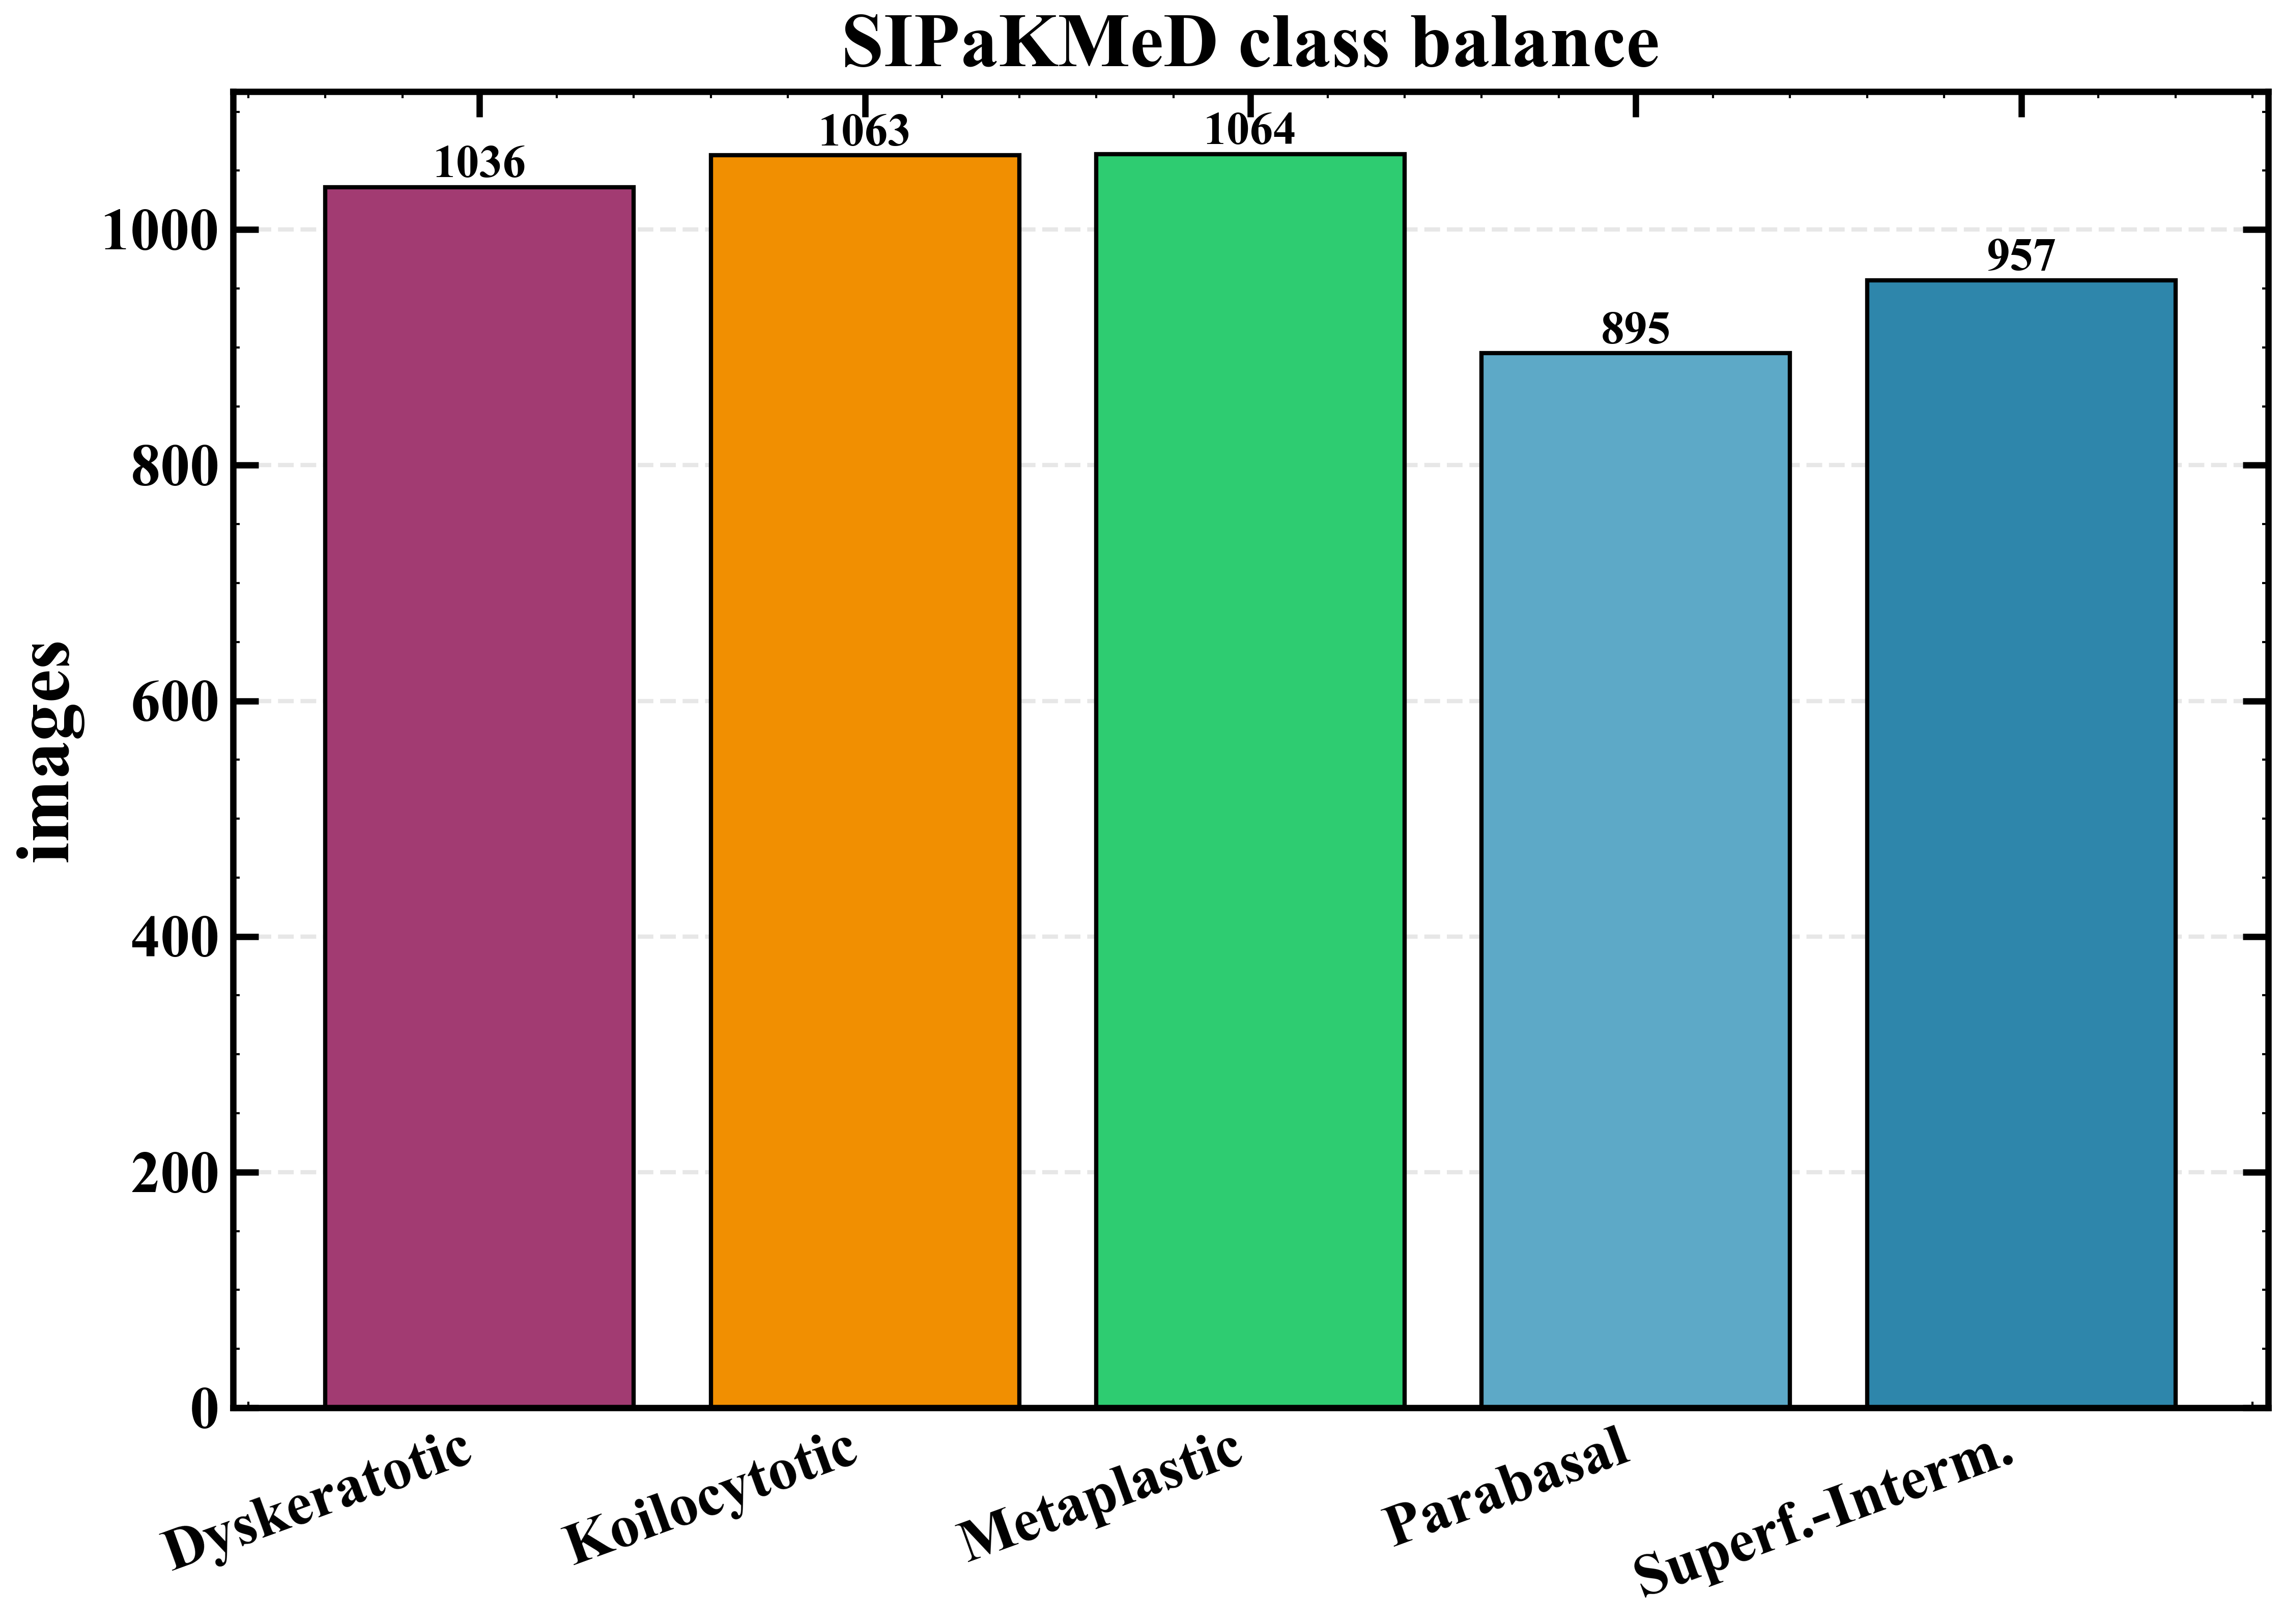
\includegraphics[width=0.40\textwidth]{eda_class_balance.png}\hfill
  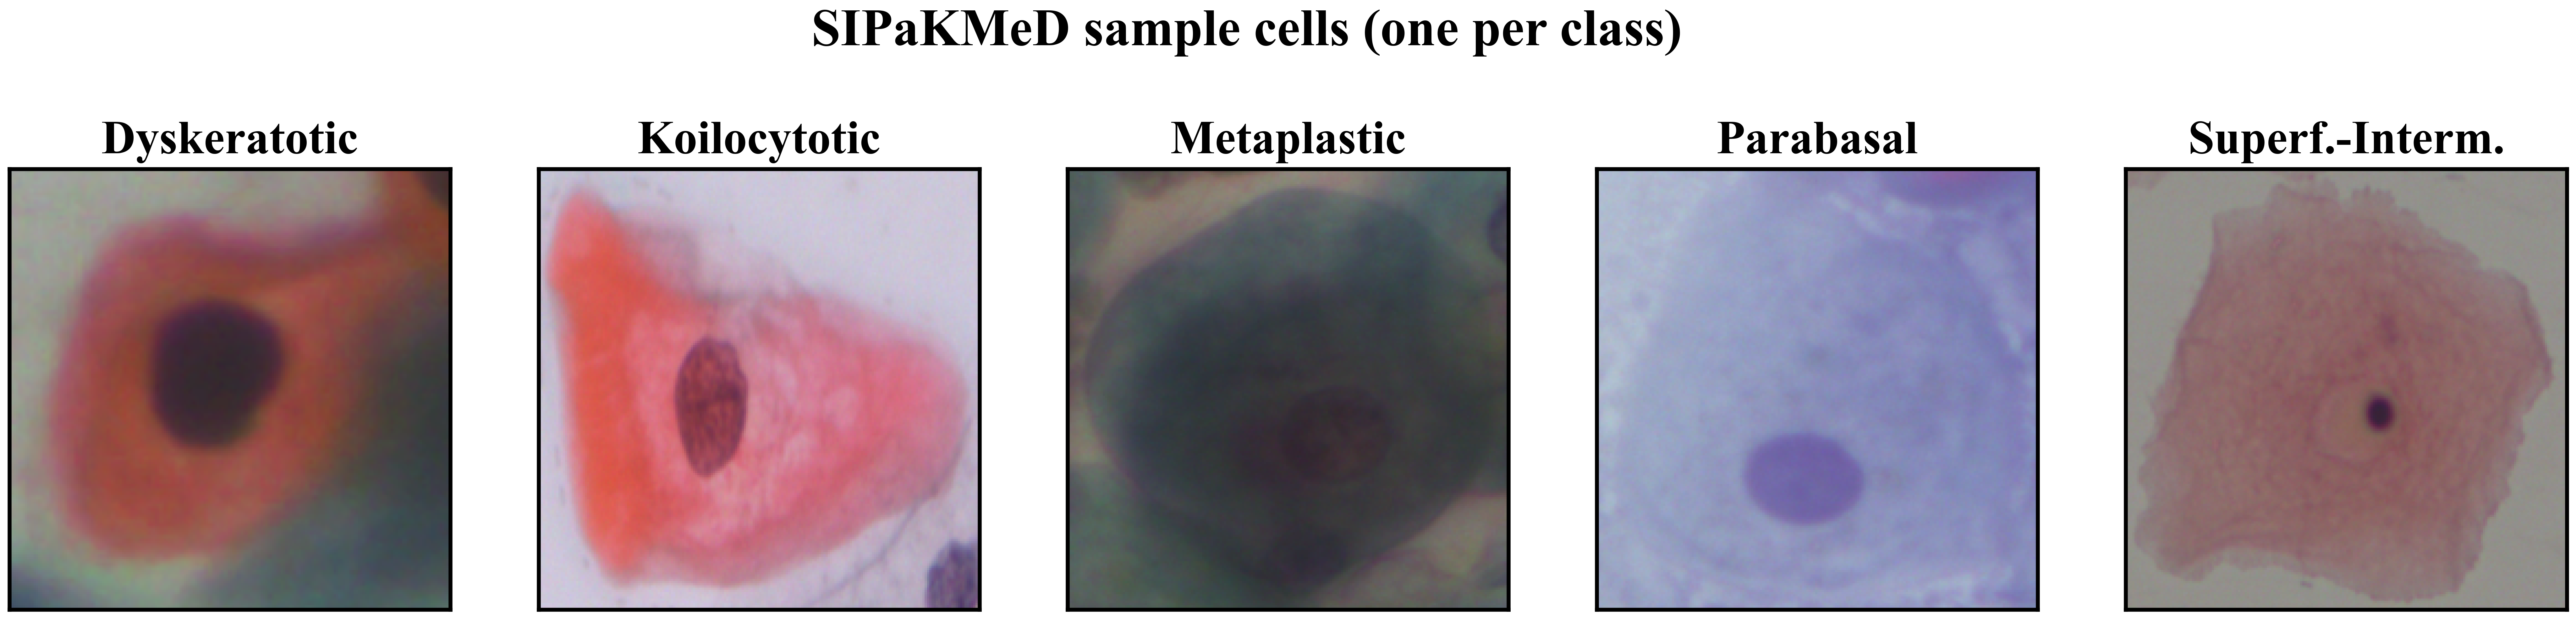
\includegraphics[width=0.56\textwidth]{eda_sample_cells.png}
  \caption{\textbf{Exploratory data analysis of \sipakmed.} Left: per-class image counts (mild
  imbalance, ratio $1.19$). Right: representative cells across the five morphology classes.}
  \label{fig:eda}
\end{figure*}

\subsection{Preprocessing and augmentation}
\label{sec:preproc}
Images are decoded to RGB, resized to $380\!\times\!380$ (the B4 native resolution, used for both
teacher and student), and channel-normalised with ImageNet statistics~\cite{deng2009imagenet}.
Train-time augmentation is cytology-appropriate---cells have \emph{no canonical orientation}, so we
apply random horizontal and vertical flips ($p{=}0.5$ each), random rotation ($\pm72^{\circ}$), and
mild random affine scaling ($0.9\!-\!1.1$). We deliberately avoid heavy shear, elastic warps or strong
hue shifts, which distort nuclear morphology---the very signal that separates the classes. Evaluation
(in- and cross-distribution) uses resize and normalisation only, with no augmentation.

\subsection{Architecture}
\label{sec:arch}
Both models are EfficientNets~\cite{tan2019efficientnet} with ImageNet-pretrained backbones: a B4
teacher ($18.5$\,M parameters) and a B0 student ($4.67$\,M). The native classifier is replaced by a
head $\mathrm{BN}\!\to\!\mathrm{Linear}(\,\cdot\,,512)\!\to\!\mathrm{ReLU}\!\to\!\mathrm{Dropout}
\!\to\!\mathrm{Linear}(512,5)$.

\subsection{Two-stage teacher and knowledge distillation}
\label{sec:train}
The teacher is trained in two stages with Adam and class-weighted cross-entropy (weight
$\propto 1/\text{count}$), monitoring validation loss: \emph{stage 1} freezes the backbone (lr
$10^{-3}$, $\le 30$ epochs, ReduceLROnPlateau), \emph{stage 2} fine-tunes the whole network (lr
$10^{-5}$, $\le 50$ epochs). The student is then distilled with the Hinton
objective~\cite{hinton2015distilling}:
\begin{equation}
\begin{split}
\mathcal{L} = {}&\alpha\,\mathrm{CE}(y,z_s) \\
&+ (1-\alpha)\,T^2\,
\mathrm{KL}\!\big(\softmax(z_t/T)\,\|\,\softmax(z_s/T)\big),
\end{split}
\label{eq:kd}
\end{equation}
with temperature $T{=}4$ and $\alpha{=}0.1$ (so the soft teacher signal dominates), Adam (lr
$5\!\times\!10^{-5}$, $\le 40$ epochs), monitoring validation accuracy. Training uses BF16 mixed
precision on a single $16$\,GB consumer GPU, batch size $32$, seed $42$, and a per-class stratified
$80/20$ train/validation split ($4{,}012$ train, $1{,}003$ validation). The teacher converges in
$71$ epochs ($30$ frozen $+$ $41$ fine-tuning, early-stopped) and the student in $34$ epochs; both
validation curves track training, indicating no overfitting (\cref{sec:exp}). We flag here---and
quantify in \cref{sec:analysis}---that this random per-cell split leaks same-field-of-view cells
across train and validation, making the internal estimate optimistic.
